\documentclass[dvips, lscape]{foils}
%\documentclass[dvips, french]{slides}
\textwidth 18.5cm
\textheight 25cm 
\topmargin -1cm 
\oddsidemargin  -1cm 
\evensidemargin  -1cm

% Maths
\usepackage{amsfonts, amsmath, amssymb}

\newcommand{\coefbin}[2]{\left( 
    \begin{array}{c} #1 \\ #2 \end{array} 
  \right)}
\newcommand{\Bcal}{\mathcal{B}}
\newcommand{\Ccal}{\mathcal{C}}
\newcommand{\Dcal}{\mathcal{D}}
\newcommand{\Ecal}{\mathcal{E}}
\newcommand{\Gcal}{\mathcal{G}}
\newcommand{\Mcal}{\mathcal{M}}
\newcommand{\Ncal}{\mathcal{N}}
\newcommand{\Pcal}{\mathcal{P}}
\newcommand{\Qcal}{\mathcal{Q}}
\newcommand{\Lcal}{\mathcal{L}}
\newcommand{\Tcal}{\mathcal{T}}
\newcommand{\Ucal}{\mathcal{U}}
\newcommand{\alphabf}{\mbox{\mathversion{bold}{$\alpha$}}}
\newcommand{\betabf}{\mbox{\mathversion{bold}{$\beta$}}}
\newcommand{\gammabf}{\mbox{\mathversion{bold}{$\gamma$}}}
\newcommand{\mubf}{\mbox{\mathversion{bold}{$\mu$}}}
\newcommand{\Pibf}{\mbox{\mathversion{bold}{$\Pi$}}}
\newcommand{\psibf}{\mbox{\mathversion{bold}{$\psi$}}}
\newcommand{\Thetabf}{\mbox{\mathversion{bold}{$\Theta$}}}
\newcommand{\taubf}{\mbox{\mathversion{bold}{$\tau$}}}
\newcommand{\Cbf}{{\bf C}}
\newcommand{\Ebf}{{\bf E}}
\newcommand{\Gbf}{{\bf G}}
\newcommand{\Hbf}{{\bf H}}
\newcommand{\Ibf}{{\bf I}}
\newcommand{\mbf}{{\bf m}}
\newcommand{\Rbf}{{\bf R}}
\newcommand{\Sbf}{{\bf S}}
\newcommand{\Tbf}{{\bf T}}
\newcommand{\ubf}{{\bf u}}
\newcommand{\Ubf}{{\bf U}}
\newcommand{\vbf}{{\bf v}}
\newcommand{\Vbf}{{\bf V}}
\newcommand{\xbf}{{\bf x}}
\newcommand{\Xbf}{{\bf X}}
\newcommand{\Ybf}{{\bf Y}}
\newcommand{\Zbf}{{\bf Z}}
\newcommand{\Esp}{{\mathbb E}}
\newcommand{\Var}{{\mathbb V}}
\newcommand{\Cov}{{\mathbb C}\mbox{ov}}
\newcommand{\Ibb}{{\mathbb I}}
\newcommand{\Rbb}{\mathbb{R}}

% sommes
\newcommand{\sumk}{\sum_k}
\newcommand{\sumt}{\sum_{t \in I_k}}
\newcommand{\sumth}{\sum_{t=t_{k-1}^{(h)}+1}^{t_k^{(h)}}}
\newcommand{\sump}{\sum_{p=1}^{P}}
\newcommand{\suml}{\sum_{\ell=1}^{P}}
\newcommand{\sumtau}{\sum_k \widehat{\tau}_{kp}}

% Couleur et graphiques
\usepackage{color}
\usepackage{graphics}
\usepackage{epsfig} 
\usepackage{pstcol}

% Texte
\usepackage{lscape}
\usepackage{../../../../Latex/fancyheadings, rotating, enumerate}
%\usepackage[french]{babel}
\usepackage[latin1]{inputenc}
\definecolor{darkgreen}{cmyk}{0.5, 0, 0.5, 0.5}
\definecolor{orange}{cmyk}{0, 0.6, 0.8, 0}
\definecolor{jaune}{cmyk}{0, 0.5, 0.5, 0}
\newcommand{\textblue}[1]{\textcolor{blue}{#1}}
\newcommand{\textred}[1]{\textcolor{red}{#1}}
\newcommand{\textgreen}[1]{\textcolor{green}{ #1}}
\newcommand{\textlightgreen}[1]{\textcolor{green}{#1}}
%\newcommand{\textgreen}[1]{\textcolor{darkgreen}{#1}}
\newcommand{\textorange}[1]{\textcolor{orange}{#1}}
\newcommand{\textyellow}[1]{\textcolor{yellow}{#1}}
\newcommand{\refer}[2]{\textgreen{[{\sl #1, #2}]}}
\newcommand{\emphase}[1]{\textblue{#1}}

% Sections
%\newcommand{\chapter}[1]{\centerline{\LARGE \textblue{#1}}}
% \newcommand{\section}[1]{\centerline{\Large \textblue{#1}}}
% \newcommand{\subsection}[1]{\noindent{\Large \textblue{#1}}}
% \newcommand{\subsubsection}[1]{\noindent{\large \textblue{#1}}}
% \newcommand{\paragraph}[1]{\noindent {\textblue{#1}}}
% Sectionsred
\newcommand{\chapter}[1]{
  \addtocounter{chapter}{1}
  \setcounter{section}{0}
  \setcounter{subsection}{0}
  {\centerline{\LARGE \textblue{\arabic{chapter} - #1}}}
  }
\newcommand{\section}[1]{
  \addtocounter{section}{1}
  \setcounter{subsection}{0}
  {\centerline{\Large \textblue{\arabic{chapter}.\arabic{section} - #1}}}
  }
\newcommand{\subsection}[1]{
  \addtocounter{subsection}{1}
  {\noindent{\large \textblue{#1}}}
  }
% \newcommand{\subsection}[1]{
%   \addtocounter{subsection}{1}
%   {\noindent{\large \textblue{\arabic{chapter}.\arabic{section}.\arabic{subsection} - #1}}}
%   }
\newcommand{\paragraph}[1]{\noindent{\textblue{#1}}}

%%%%%%%%%%%%%%%%%%%%%%%%%%%%%%%%%%%%%%%%%%%%%%%%%%%%%%%%%%%%%%%%%%%%%%
%%%%%%%%%%%%%%%%%%%%%%%%%%%%%%%%%%%%%%%%%%%%%%%%%%%%%%%%%%%%%%%%%%%%%%
%%%%%%%%%%%%%%%%%%%%%%%%%%%%%%%%%%%%%%%%%%%%%%%%%%%%%%%%%%%%%%%%%%%%%%
%%%%%%%%%%%%%%%%%%%%%%%%%%%%%%%%%%%%%%%%%%%%%%%%%%%%%%%%%%%%%%%%%%%%%%
\begin{document}
%%%%%%%%%%%%%%%%%%%%%%%%%%%%%%%%%%%%%%%%%%%%%%%%%%%%%%%%%%%%%%%%%%%%%%
%%%%%%%%%%%%%%%%%%%%%%%%%%%%%%%%%%%%%%%%%%%%%%%%%%%%%%%%%%%%%%%%%%%%%%
%%%%%%%%%%%%%%%%%%%%%%%%%%%%%%%%%%%%%%%%%%%%%%%%%%%%%%%%%%%%%%%%%%%%%%
%%%%%%%%%%%%%%%%%%%%%%%%%%%%%%%%%%%%%%%%%%%%%%%%%%%%%%%%%%%%%%%%%%%%%%
\landscape
\newcounter{chapter}
\newcounter{section}
\newcounter{subsection}
\setcounter{chapter}{0}
\headrulewidth 0pt 
\pagestyle{fancy} 
\cfoot{}
\rfoot{\begin{rotate}{90}{
      \hspace{1cm} \tiny S. Robin: Statistical analysis of CGH data
      }\end{rotate}}
\rhead{\begin{rotate}{90}{
      \hspace{-.5cm} \tiny \thepage
      }\end{rotate}}

%%%%%%%%%%%%%%%%%%%%%%%%%%%%%%%%%%%%%%%%%%%%%%%%%%%%%%%%%%%%%%%%%%%%%%
%%%%%%%%%%%%%%%%%%%%%%%%%%%%%%%%%%%%%%%%%%%%%%%%%%%%%%%%%%%%%%%%%%%%%%
\begin{center}
  \textblue{\LARGE Statistical Analysis of CGH Arrays}

   \vspace{1cm}
   {\large S. Robin} \\
   robin@inapg.inra.fr
   
   {UMR AgroParisTech / INRA: Math�matique et Informatique Appliqu�es}
   \\
   {SSB group: genome.jouy.inra.fr/ssb/}
   
    \vspace{1cm}
    { ACI-IMPBIO } \\
    {Paris, 04 - 10 - 2007}
\end{center}

%\vspace{2cm}
\paragraph{Outline} \\
\\
\begin{tabular}{ll}
  1 - Detecting chromosomal aberrations
  & 4 - Multiple arrays analysis \\ 
  \\
  2 - Looking for breakpoints
  & 5 - Looking for common aberrations \\
  \\
  3 - Segments classification
  & 6 - Future work
\end{tabular}


%%%%%%%%%%%%%%%%%%%%%%%%%%%%%%%%%%%%%%%%%%%%%%%%%%%%%%%%%%%%%
%%%%%%%%%%%%%%%%%%%%%%%%%%%%%%%%%%%%%%%%%%%%%%%%%%%%%%%%%%%%%
\newpage
\chapter{Detecting chromosomal aberrations}
%%%%%%%%%%%%%%%%%%%%%%%%%%%%%%%%%%%%%%%%%%%%%%%%%%%%%%%%%%%%%
%%%%%%%%%%%%%%%%%%%%%%%%%%%%%%%%%%%%%%%%%%%%%%%%%%%%%%%%%%%%%

% %%%%%%%%%%%%%%%%%%%%%%%%%%%%%%%%%%%%%%%%%%%%%%%%%%%%%%%%%%
% \vspace{1cm}
% \section{Aberration at the chromosomic scale}
% %%%%%%%%%%%%%%%%%%%%%%%%%%%%%%%%%%%%%%%%%%%%%%%%%%%%%%%%%%

% Known effects of big size chromosomal aberrations  (ex:
% trisomy).

% \centerline{$\rightarrow$ experimental tool: \textblue{Karyotype}
%   (Resolution $\sim$ chromosome)} 

% $$
% \epsfig{file = ../Figures/Karyotype.ps, clip=,
%   bbllx=158, bblly=560, bburx=452, bbury=778, scale=1.2}
% $$

%%%%%%%%%%%%%%%%%%%%%%%%%%%%%%%%%%%%%%%%%%%%%%%%%%%%%%%%%%
% \newpage
\bigskip
\section{Within chromosome aberration}
%%%%%%%%%%%%%%%%%%%%%%%%%%%%%%%%%%%%%%%%%%%%%%%%%%%%%%%%%%
\begin{itemize}
\item \vspace{-0.5cm} Change of scale: what are the effects of small size DNA
  sequences deletions/amplifications?\\
%  \\
  \centerline{$\rightarrow$ experimental tool:
    \textblue{"conventional" CGH} (resolution $\sim$ 10Mb).}
\item \vspace{-0.5cm} CGH = Comparative Genomic Hybridization: method for the
  comparative measurement of relative DNA copy numbers between two
  samples (normal/disease, test/reference).\\ 
%  \\
  \centerline{$\rightarrow$ Application of the \textblue{microarray}
    technology to CGH (resolution $\sim$ 100kb).}
  $$
  \epsfig{file = ../Figures/CGHarray.ps, clip=,
    bbllx=113, bblly=564, bburx=497, bbury=778, scale=1.1}
  $$
\end{itemize}

%%%%%%%%%%%%%%%%%%%%%%%%%%%%%%%%%%%%%%%%%%%%%%%%%%%%%%%%%%%%%
\newpage
\section{Microarray technology in its principle }
%%%%%%%%%%%%%%%%%%%%%%%%%%%%%%%%%%%%%%%%%%%%%%%%%%%%%%%%%%%%%
\vspace{-1cm}
$$
\epsfig{file = ../Figures/principe_CGH.eps, clip=,
  bbllx=0, bblly=41, bburx=700, bbury=478, scale=0.9}
$$

%%%%%%%%%%%%%%%%%%%%%%%%%%%%%%%%%%%%%%%%%%%%%%%%%%%%%%%%%%%%%
\newpage
\section{Interpretation of a CGH profile }
%%%%%%%%%%%%%%%%%%%%%%%%%%%%%%%%%%%%%%%%%%%%%%%%%%%%%%%%%%%%%

\noindent
\begin{tabular}{cc}
  \begin{tabular}{p{7cm}}
    \paragraph{Data size.} \\
    \\
    Few thousands points / genome\\
    \\
    Few hundreds points / chromosome\\
    \\ \\ \\ \\
    \paragraph{A dot on the graph = }
  \end{tabular} 
  &
  \begin{tabular}{c}
    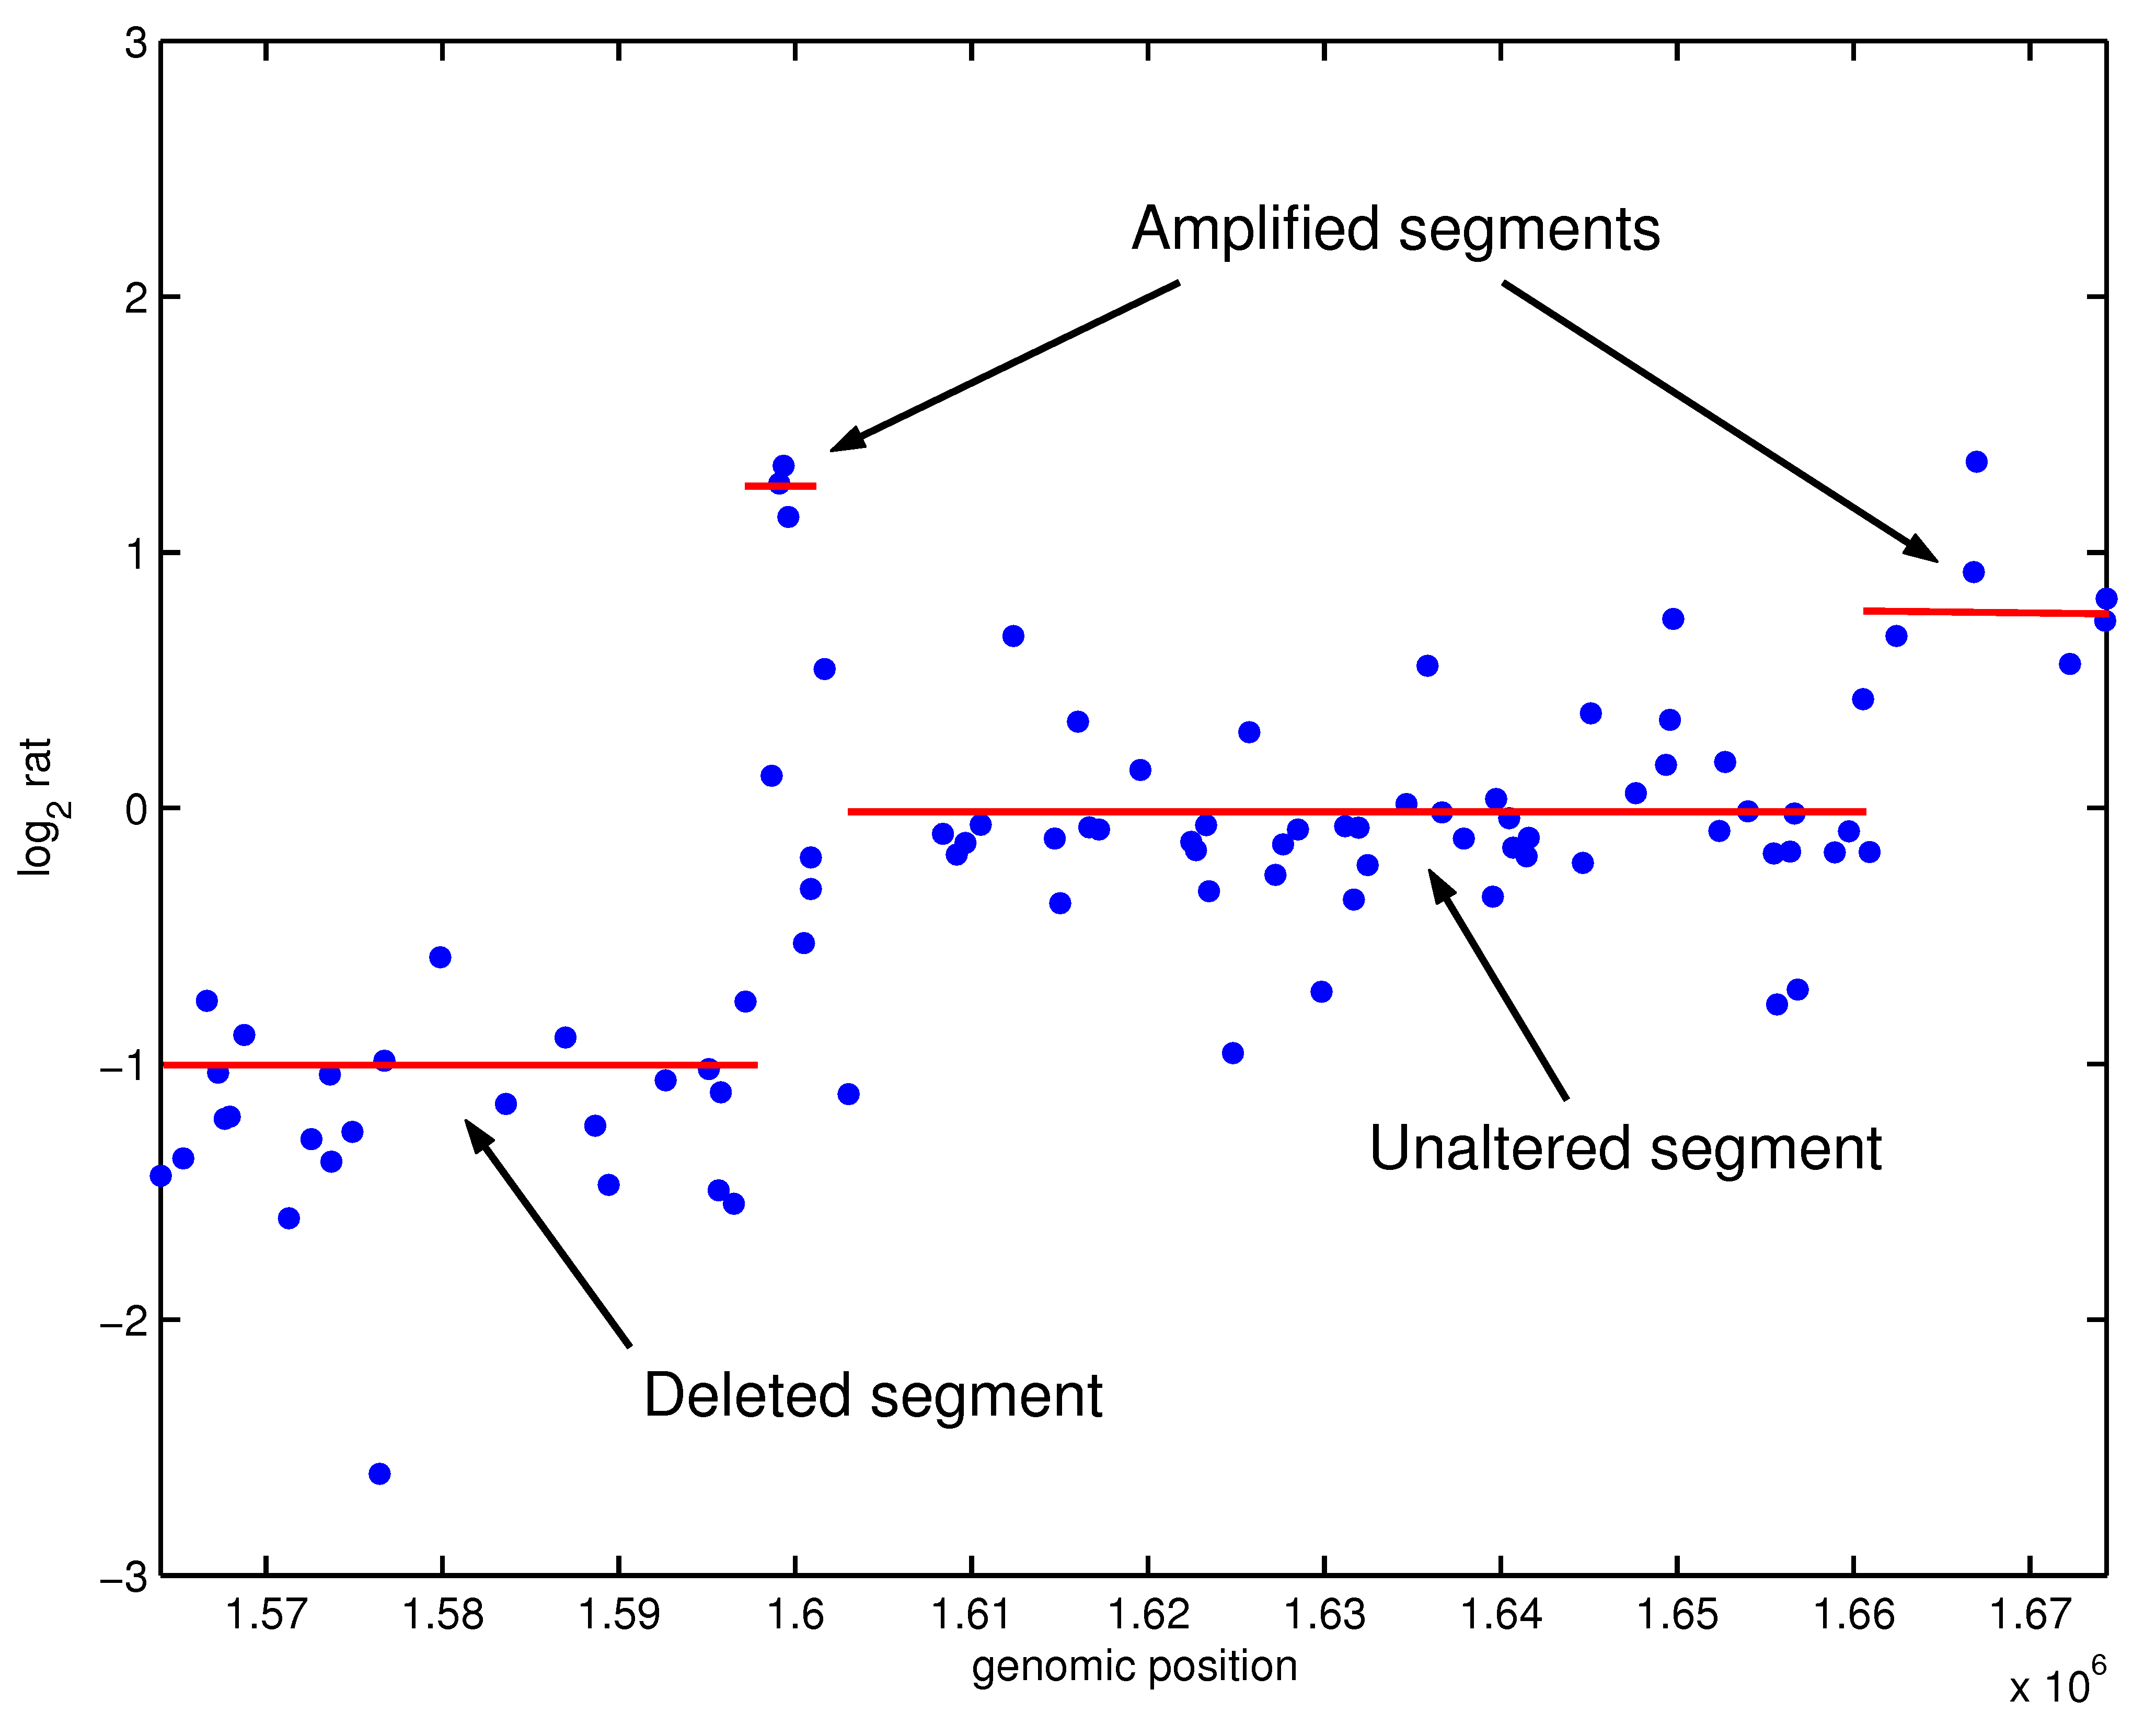
\epsfig{file = ../Figures/profile_example.eps, clip=,
      bbllx=60, bblly=196, bburx=543, bbury=586, width=16cm}
  \end{tabular} 
\end{tabular} 
\vspace{-0.25cm}
$$
\log_2 \left\{ \frac{\text{ $\sharp$ copies of BAC(t) in the test
      genome }}{\text{$\sharp$ copies of BAC(t) in the reference
      genome}}\right\}
$$


%%%%%%%%%%%%%%%%%%%%%%%%%%%%%%%%%%%%%%%%%%%%%%%%%%%%%%%%%%%%%
%%%%%%%%%%%%%%%%%%%%%%%%%%%%%%%%%%%%%%%%%%%%%%%%%%%%%%%%%%%%%
\newpage
\chapter{Looking for breakpoints}
%%%%%%%%%%%%%%%%%%%%%%%%%%%%%%%%%%%%%%%%%%%%%%%%%%%%%%%%%%%%%
%%%%%%%%%%%%%%%%%%%%%%%%%%%%%%%%%%%%%%%%%%%%%%%%%%%%%%%%%%%%%

%%%%%%%%%%%%%%%%%%%%%%%%%%%%%%%%%%%%%%%%%%%%%%%%%%%%%%%%%%
\bigskip
%\section{What to we have in mind?}
\section{Statistical model} 
%%%%%%%%%%%%%%%%%%%%%%%%%%%%%%%%%%%%%%%%%%%%%%%%%%%%%%%%%%

\begin{itemize}
\item At position $t$, there exists a 'true' log-ratio, which depends
  on the relative copy number.
\item The value of the true log-ratio is affected by abrupt changes:
                                %\vspace{-0.5cm}
  $$
  \epsfig{file = ../Figures/FigSeg_Intro_bis.eps, clip=, bbllx=90,
    bblly=300, bburx=540, bbury=400, scale = 1.2}
  $$
  Positions \emphase{$t_1$, $t_2$, ..} are called
  \emphase{breakpoints}. \emphase{$\mu_k$} is the true log-ratio in
  segment \emphase{$I_k$}.
\item The observed signal $Y_t$ is noisy:
  $$
  \mbox{if } t \in I_k: 
  \qquad Y_t \sim \Ncal(\mu_k, \sigma^2_{(k)}), 
  \qquad \{Y_t\}_t \mbox{ independent}.
  $$
\end{itemize}
%   where $\lambda_t$ is the true log-ratio 
%   and $E_t$ is a noise (typically, $E_t \sim \Ncal(0, \sigma^2)$).


% %%%%%%%%%%%%%%%%%%%%%%%%%%%%%%%%%%%%%%%%%%%%%%%%%%%%%%%%%%
% \newpage
% \section{Statistical model} 
% %%%%%%%%%%%%%%%%%%%%%%%%%%%%%%%%%%%%%%%%%%%%%%%%%%%%%%%%%%
% \vspace{-0.5cm}\begin{itemize}
% \item The breakpoints define a partition of the data into $K$
%   segments of size $n_k$:
%   $$
%   I_k=\{t, t \in ]t_{k-1},t_k]\}, 
%   \qquad
%   Y^k=\{Y_t, t \in I_k\}.
%   $$
% \item Suppose that these parameters are constant between two changes
%   \refer{Picard et al.}{2005}: 
%   $$
%   \mbox{if position $t$ is in segments $I_k$,} \qquad Y_t = \mu_k +
%   E_t \sim \Ncal(\mu_k,\sigma_{(k)}^2).
%   $$
% \item The parameters of this model are: 
%   $$
%   T  =  (t_1, ..., t_{K-1}),
%   \qquad
%   \Theta  = (\theta_1,\hdots,\theta_K), \quad \theta_k=(\mu_k,\sigma_{(k)}^2).
%   $$
% \end{itemize}
% Breakpoints detection aims at studying the \textblue{spatial structure
%   of the signal}.

%%%%%%%%%%%%%%%%%%%%%%%%%%%%%%%%%%%%%%%%%%%%%%%%%%%%%%%%%%
\newpage
\subsection{Segmentation as a linear model}
%%%%%%%%%%%%%%%%%%%%%%%%%%%%%%%%%%%%%%%%%%%%%%%%%%%%%%%%%%

The model defined above can be stated in the \emphase{general linear
  model} framework:
$$
\Ybf = \Tbf \mubf + \Ebf
$$
where
\begin{itemize}
\item $\Ybf$ is the $n$-vector containing the profile, 
\item $\Tbf$ is the $N \times K$ \emphase{segmentation matrix} that
  associates each position to a segment,
\item $\mubf$ is the $K$-vector containing the means of each segment, 
\item $\Ebf$ is the $n$-vector containing the random noise
  (i.i.d. $\sim \Ncal(0, \sigma^2)$).
\end{itemize}

\paragraph{Remark.}
In our case, the matrix \emphase{$\Tbf$ has to be estimated}.

%%%%%%%%%%%%%%%%%%%%%%%%%%%%%%%%%%%%%%%%%%%%%%%%%%%%%%%%%%
\newpage
\subsection{Estimating the parameters}
%%%%%%%%%%%%%%%%%%%%%%%%%%%%%%%%%%%%%%%%%%%%%%%%%%%%%%%%%%

\paragraph{Log-Likelihood} (with a constant variance $\sigma^2$):
\begin{eqnarray*}
\Lcal_K(T, \Theta) 
% & = & \sum_{k=1}^K \log \phi(\{Y_t\}_{t \in I_k};
% \theta_k) \quad = \quad \sum_{k=1}^K \sum_{t \in I_k}\log \phi(Y_t;
% \theta_k) \\ 
& = & -n \log \sigma^2 - \frac1{\sigma^2} \sum_{k=1}^K \sum_{t \in
  I_k} (Y_t - \mu_k)^2 + \mbox{cst}. 
\end{eqnarray*}

\begin{itemize}
\item Because the data are supposed to be independent, the
  log-likelihood is \emphase{additive} (i.e. sum over all the segments).
% \item Because the data are supposed to be Gaussian, maximum likelihood
%   estimation is equivalent to least square fitting.
\item Given the breakpoint position, the estimates of $\mu_k$ and
  $\sigma^2_{(k)}$ are straightforward:
  $$
  \widehat{\mu}_k = \frac1{n_k} \sum_{t \in I_k} Y_t 
  \quad \mbox{and} \quad
  \widehat{\sigma}^2 =  \frac1{n} \sum_{k=1}^K \sum_{t \in I_k} (Y_t -
  \widehat{\mu}_k)^2 
  \quad \mbox{or} \quad
  \widehat{\sigma}^2_k = \frac1{n_k} \sum_{t \in I_k} (Y_t -
  \widehat{\mu}_k)^2.
  $$
\end{itemize}

%%%%%%%%%%%%%%%%%%%%%%%%%%%%%%%%%%%%%%%%%%%%%%%%%%%%%%%%%%
\newpage
\subsection{How to find the breakpoints?}

When the number of segments $K$ is known , we have to minimize
$$
J_k(1, n) = \sum_{k=1}^K \sum_{t \in I_k} (Y_t - \widehat{\mu}_k)^2.
$$
\begin{itemize}
\item The $\coefbin{n-1}{K-1}$ possible choices for the positions of
  the breakpoints $t_1, t_2, \dots, t_{K-1}$ can not be explored for
  large $n$ and $K$
\item $\sum_{t \in I_k} (Y_t - \widehat{\mu}_k)^2$ can be viewed as
  the \emphase{'cost' of segment $I_k$}, i.e. the cost of gathering
  data $Y_{t_{k-1}+1}$ to $Y_{t_{k+1}}$ into a single segment.
\item The optimization problem is actually a shortest path problem
  that can be solved thanks to \emphase{dynamic programming}
  \refer{Picard et al.}{2005}.
\end{itemize}


%%%%%%%%%%%%%%%%%%%%%%%%%%%%%%%%%%%%%%%%%%%%%%%%%%%%%%%%%%
\newpage
\subsection{One last problem: the selection of $K$}

\noindent
\begin{tabular}{cc}
  \begin{tabular}{p{10cm}}
    \begin{itemize}
    \item $J_K$ decreases when $K$ (\emphase{complexity}) increases.
    \item Standard criteria such as AIC or BIC are
      \emphase{not valid}.
    \item \emphase{Penalty function}: $pen(K) = $ $K+1$ or $2K$.
    \item We look for the minimum of
      $$
      J_k + \beta pen(K)
      $$
      where $\beta$ is given \refer{Lebarbier}{2005} or adaptively
      estimated \refer{Lavielle}{2003}.
    \end{itemize}
  \end{tabular}
  &
  \begin{tabular}{c}
    \epsfig{file = ../Figures/Select_K.ps, clip=, bbllx=146, bblly=529,
      bburx=464, bbury=777, width=12cm, height=12cm} 
  \end{tabular}
\end{tabular}

%%%%%%%%%%%%%%%%%%%%%%%%%%%%%%%%%%%%%%%%%%%%%%%%%%%%%%%%%%
\newpage
\section{Example of segmentation on array CGH data}
%%%%%%%%%%%%%%%%%%%%%%%%%%%%%%%%%%%%%%%%%%%%%%%%%%%%%%%%%%

\paragraph{Are the variances $\sigma^2_k$ homogeneous?} BT474 cell
line, chromosome 9: 
$$
\begin{tabular}{cc}
  Homogeneous variances & Heterogeneous variances \\
  \multicolumn{2}{c}{$K=4$ segments} \\
  \epsfig{file = ../Figures/bt474_c9_seg_homo_K4.eps, clip=, scale=0.7} &
  \epsfig{file = ../Figures/bt474_c9_seg_hetero_K4.eps, clip=, scale=0.7} \\
\end{tabular}
$$

%%%%%%%%%%%%%%%%%%%%%%%%%%%%%%%%%%%%%%%%%%%%%%%%%%%%%%%%%%
\newpage
\paragraph{Adaptive choice of the number of segments.} BT474 cell
line, chromosome 1:
$$
\begin{tabular}{cc}
  Homogeneous variances & Heterogeneous variances \\
  $\widehat{K} = 10$  segments & $\widehat{K} = 2$ segments \\
  \epsfig{file = ../Figures/bt474_c1_seg_homo_K10.eps, clip=, scale=0.7} &
  \epsfig{file = ../Figures/bt474_c1_seg_hetero_K2.eps, clip=, scale=0.7} \\
\end{tabular}
$$
Homogeneous variances result in smaller segments.

%%%%%%%%%%%%%%%%%%%%%%%%%%%%%%%%%%%%%%%%%%%%%%%%%%%%%%%%%%
\newpage
\subsection{Comparative study} 

\vspace{-0.5cm}
\paragraph{Lai \& al. (Bioinformatics, 05).} On both synthetic and
real data (GBM brain tumor data), the dynamic programming approach
outperfoms other methods available at that time.
$$
%\epsfig{file = ../Figures/LPJ05-Fig1.eps, clip=, scale=1.2}
%\epsfig{file = ../Figures/LPJ05-Fig3.eps, clip=, scale=1.2}
\epsfig{file = ../Figures/LPJ05-Fig4.eps, clip=, scale=1.2}
$$

%%%%%%%%%%%%%%%%%%%%%%%%%%%%%%%%%%%%%%%%%%%%%%%%%%%%%%%%%%%%%
%%%%%%%%%%%%%%%%%%%%%%%%%%%%%%%%%%%%%%%%%%%%%%%%%%%%%%%%%%%%%
\newpage
\chapter{Segments classification}
%%%%%%%%%%%%%%%%%%%%%%%%%%%%%%%%%%%%%%%%%%%%%%%%%%%%%%%%%%%%%
%%%%%%%%%%%%%%%%%%%%%%%%%%%%%%%%%%%%%%%%%%%%%%%%%%%%%%%%%%%%%

\bigskip
\paragraph{Considering biologists objective and the need for a new
  model.}
$$
\begin{tabular}{cc}
  \epsfig{file = ../Figures/FigSegClas-1.eps, clip=, scale=0.7} &
  \epsfig{file = ../Figures/FigSegClas-2.eps, clip=, scale=0.7} \\
\end{tabular}
$$
We'd like segments of same type ('normal', 'deleted', amplified')
to be gathered into classes.
% $$
% \epsfig{file = ../Figures/nouveau_modele.ps, angle=270, clip=,
%   bbllx=92, bblly=47, bburx=484, bbury=828, scale=0.9}
% $$

%%%%%%%%%%%%%%%%%%%%%%%%%%%%%%%%%%%%%%%%%%%%%%%%%%%%%%%%%%
\newpage
\section{A segmentation-clustering model}
%%%%%%%%%%%%%%%%%%%%%%%%%%%%%%%%%%%%%%%%%%%%%%%%%%%%%%%%%%

\begin{itemize}
\item We suppose that there exists a \textblue{secondary unobserved
    structure} that clusters the $K$ segments into $P$ classes with
  proportions $\pi_1,...,\pi_P$:
% \item We introduce hidden variables, $Z_{kp}$ indicators of the
%   class of origin of \textblue{segment $k$}.
% \item These variables are supposed independent, with multinomial
%   distribution:
  $$
  \pi_p = \mbox{proportion of class $p$}, 
  \qquad \sum_p \pi_p=1.
%   (Z_{k1},\hdots,Z_{kP}) \sim \mathcal{M}(1;\pi_1,\hdots,\pi_P).
  $$
\item Conditionally to the class to which the segment belongs, we know
  the distribution of $Y$:
  $$
  t \in I_k, k \in p \qquad \Rightarrow \qquad Y_t \sim \Ncal(m_p, s_p^2).
%   Y^k|Z_{kp}=1 \sim \Ncal({\bf 1}_{n_k} m_p, s_p^2 {\bf I}_{n_k}).
  $$
  \refer{Picard et al.}{2007}
%\item It is a model of \textblue{segmentation/clustering}.
\end{itemize}

The parameters of this model are
\begin{eqnarray*}
  \mbox{the breakpoint positions:} & \quad & T = \{t_1, ..., t_{K-1}\} ,\\
  \mbox{the mixture characteristics:} & \quad & \Psi = (\{\pi_p\}, \{m_p\},
  \{s^2_p\}). 
\end{eqnarray*}

%%%%%%%%%%%%%%%%%%%%%%%%%%%%%%%%%%%%%%%%%%%%%%%%%%%%%%%%%%
\newpage
\subsection{Matrix form}
%%%%%%%%%%%%%%%%%%%%%%%%%%%%%%%%%%%%%%%%%%%%%%%%%%%%%%%%%%

This model can written as
$$
\Ybf = \Tbf \Cbf \mbf + \Ebf
$$
where
\begin{itemize}
\item $\Cbf$ is the $K \times P$ \emphase{classification matrix} that
  assigns each segment to a class,
\item $\mbf$ is the $P$ vector containing the mean of each class.
\end{itemize}

\paragraph{Remarks.}
\begin{itemize}
\item \vspace{-0.5cm} This model is not linear anymore. 
\item \vspace{-0.5cm} $\Cbf$ represents the unobserved part of this
  \emphase{incomplete data model}.
\item \vspace{-0.5cm} Two levels of statistical units: the positions
  ($t$) and the segments($k$).
\end{itemize}

% %%%%%%%%%%%%%%%%%%%%%%%%%%%%%%%%%%%%%%%%%%%%%%%%%%%%%%%%%%
% \newpage
% \section{Likelihood and statistical units of the model }
% %%%%%%%%%%%%%%%%%%%%%%%%%%%%%%%%%%%%%%%%%%%%%%%%%%%%%%%%%%

% \paragraph{Mixture model of segments:} 
% \vspace{-0.5cm}    \mbox{the brakpoint positions:} \quad 
% \begin{itemize}
% \item the statistical units are segments:$Y^k$,
% \item the density of $Y^k$ is a mixture density:
%   $$
%   \log \Lcal_{KP}(T, \Psi)= \sum_{k=1}^K \log
%   f_P(Y^k;\Psi)=\sum_{k=1}^K \log \left\{ \sum_{p=1}^P \pi_p
%     \phi(Y^k;\theta_p) \right\}
%   $$
% \item \vspace{-0.5cm} If the $Y_ts$ are independent, we have:
%   $$
%   \log \Lcal_{KP}(T,\Psi) =\textcolor{red}{\sum_{k=1}^K} \log
%   \left\{ \textcolor{blue}{\sum_{p=1}^P} \pi_p \textcolor{red}{\prod_{
%         t \in I_k }}\phi(Y_t; \theta_p) \right\}. 
%   $$
%   instead of $ \log \Lcal_{P}(\Psi) =
%   \textcolor{red}{\sum_{k=1}^K} \log \left\{ \textcolor{red}{\prod_{ t
%         \in I_k }} \textcolor{blue}{\sum_{p=1}^P} \pi_p \phi(Y_t;
%     \theta_p)\right \} $ in the classical mixture model where the
%   statistical units are the elementary data $Y_t$s.
% \end{itemize}

%%%%%%%%%%%%%%%%%%%%%%%%%%%%%%%%%%%%%%%%%%%%%%%%%%%%%%%%%%
\newpage
\section{An hybrid estimation algorithm: DP-EM}
%%%%%%%%%%%%%%%%%%%%%%%%%%%%%%%%%%%%%%%%%%%%%%%%%%%%%%%%%%

\paragraph{Alternate parameters estimation with $K$ and $P$ known}
\begin{enumerate}
\item When $T$ is fixed, the \textblue{Expectation-Maximisation (EM)}
  algorithm estimates $\Psi$:
  $$
  {\Psi}^{(h+1)}=\underset{\Psi}{\arg\max} \left\{\log
    \Lcal_{KP}\left(\Psi,T^{(h)}\right) \right\}. 
  $$
%   $$
%   \log \Lcal_{KP}( {\Psi}^{(h+1)}; {T}^{(h)})
%   \geq \log \Lcal_{KP}({\Psi}^{(h)};
%   {T}^{(h)})
%   $$
\item When $\Psi$ is fixed, \textblue{Dynamic Programming (DP)}
  estimates $T$:
  $$
  {T}^{(h+1)}=\underset{T}{\arg\max} \left\{\log
    \Lcal_{KP}\left({\Psi}^{(h+1)},T\right) \right\}. 
  $$
%   $$
%   \log \Lcal_{KP}({\Psi}^{(h+1)}; {T}^{(h+1)})
%   \geq \log \Lcal_{KP}({\Psi}^{(h+1)};
%   {T}^{(h)})
%   $$
\end{enumerate} 
\paragraph{An increasing sequence  of likelihoods:}
$$\log \Lcal_{KP}({\Psi}^{(h+1)}; {T}^{(h+1)}) \geq \log \Lcal_{KP}({\Psi}^{(h)}; {T}^{(h)})$$

% %%%%%%%%%%%%%%%%%%%%%%%%%%%%%%%%%%%%%%%%%%%%%%%%%%%%%%%%%%
% \newpage
% \subsection{Mixture model when the segmentation is known}
% %%%%%%%%%%%%%%%%%%%%%%%%%%%%%%%%%%%%%%%%%%%%%%%%%%%%%%%%%%

% \paragraph{Mixture model parameters estimators.}
% \begin{eqnarray}
% \mbox{posterior probability:} \qquad \widehat{\tau}_{kp} & = & \frac{\widehat{\pi}_p \phi(Y^k; \widehat{\theta}_p)}{\suml \widehat{\pi}_{h} \phi(Y^k; \widehat{\theta}_{h})}. \nonumber
% \end{eqnarray}
% \begin{itemize}
% \item the estimator the the mixing proportions is: $\widehat{\pi}_p = \frac{\sumtau}{K}$.
% \item In the gaussian case, $\theta_p=(m_p,s_p^2)$: 
% \begin{eqnarray}
% \mbox{weighted mean:} \qquad \widehat{m}_p   &=&  \frac{\sumtau \sumt Y_t}{\sumtau n_k}, \nonumber \\
% \mbox{weighted variance:} \qquad \widehat{s}_p^2 &=&  \frac{\sumtau \sumt (Y_t- \widehat{m}_p)^2}{\sumtau n_k}. \nonumber 
% \end{eqnarray}
% \item Big size vectors will have a bigger impact in the estimation of the parameters, via the term $\sumtau n_k$ \\
% \end{itemize}

% %%%%%%%%%%%%%%%%%%%%%%%%%%%%%%%%%%%%%%%%%%%%%%%%%%%%%%%%%%
% \newpage
% \subsection{Segmentation with a fixed mixture}
% %%%%%%%%%%%%%%%%%%%%%%%%%%%%%%%%%%%%%%%%%%%%%%%%%%%%%%%%%%

% \paragraph{Back to dynamic programming}
% \begin{itemize}
% \item the incomplete mixture log-likelihood can be written as a sum of local log-likelihoods:
%   $$
%   \begin{array}{ccccc}
%     \Lcal_{KP}(T,\Psi) & = & \sumk f_P(Y^k;\Psi) 
%   \end{array}
%   $$
% \item the local log-likelihood of segment $k$ corresponds to the
%   mixture log-density of vector $Y^k$
%   $$
%   f_P(Y^k;\Psi)=\log \left\{\sum_{p=1}^P \pi_p \prod_{t \in
%       I_k} \phi(Y_t;\theta_p)\right\}.
%   $$
% \item $\log \Lcal_{KP}(T,\Psi)$ can be optimized in $T$ with $\Psi$ fixed, by dynamic programming. 
% \end{itemize}

% %%%%%%%%%%%%%%%%%%%%%%%%%%%%%%%%%%%%%%%%%%%%%%%%%%%%%%%%%%%
% \newpage
% % \section{Model selection: $K=?$, $P=?$}
% % %%%%%%%%%%%%%%%%%%%%%%%%%%%%%%%%%%%%%%%%%%%%%%%%%%%%%%%%%%%

% \subsection{Choosing the number of classes $P$} 

% \vspace{-0.5cm}
% We use the BIC criterion:
% $$
% BIC = \Lcal_{P} - \log n \times (\# \mbox{ of parameters}) / 2
% $$
% \vspace{-1cm}
% $$
% \begin{tabular}{cc}
%   Simulated sequence & $\Lcal_{KP}$ and $BIC$ criterion \\
%   \epsfig{file = ../Figures/Exemple_P2K4.eps, clip=, scale=0.7} &
%   \epsfig{file = ../Figures/Exemple_P2K4_BIC.eps, clip=, scale=0.7} \\
% \end{tabular}
% $$
% The log-likelihood $\Lcal$ (\textred{\bf ---}) always increases with
% $P$ while $BIC$ ({\bf ---}) has a maximum.

% %%%%%%%%%%%%%%%%%%%%%%%%%%%%%%%%%%%%%%%%%%%%%%%%%%%%%%%%%%%
% \newpage
% \subsection{Choosing the number of segments $K$} 

% The likelihood may decrease when $K$ increases:
% $$
% \begin{tabular}{lc}
%   \hspace{-1cm}
%   \begin{tabular}{l}
%     Simulated data: \\
%     \\
%     $f_2(Y^k;\Psi) =$ \\
%     \\
%     $0.5 \Ncal(0,1)+ 0.5 \Ncal(5,1)$ \\
%     \\
%     \\
%     Log-likelihood $\Lcal_{KP}$ \\
%     as a function of $K$ \\
%     \\
%     ($P=2$) \\
%     \\
%   \end{tabular}
%   & \begin{tabular}{c}
%     \epsfig{file = ../Figures/simulation_2.eps, clip=, scale=0.8}
%   \end{tabular}
% \end{tabular}
% $$
% $\rightarrow$ sort of self-penalization of the log-likelihood with
% respect to $K$.

%%%%%%%%%%%%%%%%%%%%%%%%%%%%%%%%%%%%%%%%%%%%%%%%%%%%%%%%%%%
\newpage
\section{BT474 cell line}
%%%%%%%%%%%%%%%%%%%%%%%%%%%%%%%%%%%%%%%%%%%%%%%%%%%%%%%%%%%

\paragraph{Interest of clustering: an easy case.} Chromosome 9:
$$
  \begin{tabular}{cc}
    Segmentation & Segmentation / Clustering \\
    \multicolumn{2}{c}{$K=4$ segments} \\
    \epsfig{file = ../Figures/bt474_c9_seg_homo_K4, clip=, scale=0.7} 
    & 
    \epsfig{file = ../Figures/bt474_c9_segclas_homo_P3K4 , clip=, scale=0.7} 
  \end{tabular}
$$
Clustering defines 'deleted', 'normal' and 'amplified' classes.

\newpage

\paragraph{Interest of clustering: a more interesting case.}
Chromosome 1:
$$
\begin{tabular}{cc}
  Segmentation & Segmentation / Clustering \\
  $K=2$ & $P=3$, $K=8$ \\
  \epsfig{file = ../Figures/bt474_c1_seg_hetero_K2.eps, clip=, scale=0.7} 
  & \epsfig{file = ../Figures/resultat_P3K8.eps , clip=, scale=0.7} 
\end{tabular}
$$
Clustering detects an outliers and captures a 'normal' segment within
a large variance region.

%%%%%%%%%%%%%%%%%%%%%%%%%%%%%%%%%%%%%%%%%%%%%%%%%%%%%%%%%%%%%
%%%%%%%%%%%%%%%%%%%%%%%%%%%%%%%%%%%%%%%%%%%%%%%%%%%%%%%%%%%%%
\newpage
\chapter{Multiple arrays analysis}
%%%%%%%%%%%%%%%%%%%%%%%%%%%%%%%%%%%%%%%%%%%%%%%%%%%%%%%%%%%%%
%%%%%%%%%%%%%%%%%%%%%%%%%%%%%%%%%%%%%%%%%%%%%%%%%%%%%%%%%%%%%

\subsection{Two examples.}

\paragraph{1 - Comparing {\sl A. Thaliana} mutants or ecotypes.}
Chromosomal rearrangement can be detected by comparing CGH profiles
observed on individual from different genotypes.

\paragraph{2 - Comparing groups of patients.}
To detect chromosomal aberration associated with a specific disease
(e.g. breast cancer), we analyse the profiles of several ill patients
jointly.

\bigskip\bigskip
\subsection{First approach: Common breakpoints.}

Assuming that all the patients of the same group have their
breakpoints at the same positions, leads to \emphase{segment a
  multivariate signal}, which can be achieved using DP.

This is doable but \emphase{biologically irrelevant}.

%%%%%%%%%%%%%%%%%%%%%%%%%%%%%%%%%%%%%%%%%%%%%%%%%%%%%%%%%%
\newpage
\subsection{Breast cancer dataset (Inst. Curie): Chromosome 8.} \\
\\
\begin{tabular}{ccc}
  & Good prognosis (53 patients) & Bad prognosis (81 patients) \\
  \hspace{-1cm}
  \begin{tabular}{p{2.5cm}} Number of breakpoints \end{tabular} &
  \begin{tabular}{c}
    \epsfig{file =
      /RECHERCHE/RUPTURES/Exposes/Figures/CurieChromo8Gp1_K.eps, clip=,
      width=10cm, height=6cm}
  \end{tabular} 
  &
  \begin{tabular}{c}
    \epsfig{file =
      /RECHERCHE/RUPTURES/Exposes/Figures/CurieChromo8Gp2_K.eps, clip=,
      width=10cm, height=6cm} 
  \end{tabular} \\
  \hspace{-1cm}
  \begin{tabular}{p{2.5cm}} Position of the breakpoints \end{tabular} &
  \begin{tabular}{c}
    \epsfig{file =
      /RECHERCHE/RUPTURES/Exposes/Figures/CurieChromo8Gp1_T.eps, clip=,
      width=10cm}
  \end{tabular} 
  &
  \begin{tabular}{c}
    \epsfig{file =
      /RECHERCHE/RUPTURES/Exposes/Figures/CurieChromo8Gp2_T.eps, clip=,
      width=10cm}
  \end{tabular} 
\end{tabular}

%%%%%%%%%%%%%%%%%%%%%%%%%%%%%%%%%%%%%%%%%%%%%%%%%%%%%%%%%%%%%
\newpage
\section{Correlated profiles}
%%%%%%%%%%%%%%%%%%%%%%%%%%%%%%%%%%%%%%%%%%%%%%%%%%%%%%%%%%%%%

\hspace{-2cm}
\begin{tabular}{cc}
  \begin{tabular}{p{12cm}}
    We want to account for \emphase{correlations between profiles}. \\ \\
    \emphase{Different probe affinities} may alter all the profiles at the same
    position. \\ \\
    Denoting $Y_{it}$ the profile of patient $i$ at position $t$
    (belonging to segment $I_{ik}$), we
    set
    $$
    Y_{it} = \mu_{ik} + U_t + E_{it}
    $$
    where $\mu_{ik}$ is the mean of segment $I_{ik}$ and
    \emphase{$U_t$ is the random effect of probe $t$}: 
    $$
    \{E_{it}\} \mbox{ iid } \Ncal(0, \sigma^2),  
    \quad
    \{U_t\} \mbox{ iid } \Ncal(0, \gamma^2).  
    $$
  \end{tabular}
  &
  \begin{tabular}{l}
    \epsfig{file = ../Figures/nakao-mat.txt-MixSeg.eps, width=11cm,
    height=14cm, bbllx=90, bblly=220, bburx=380, bbury=590, clip=}
  \end{tabular}
\end{tabular}

%%%%%%%%%%%%%%%%%%%%%%%%%%%%%%%%%%%%%%%%%%%%%%%%%%%%%%%%%%%%%
\newpage
\section{Mixed segmentation model}
%%%%%%%%%%%%%%%%%%%%%%%%%%%%%%%%%%%%%%%%%%%%%%%%%%%%%%%%%%%%%

\paragraph{Covariance between profiles.}
$$
\Cov(Y_{it}, Y_{i't'}) = \Cov(U_t + E_{it}, U_{t'} + E_{i't'}) = 
\left\{
  \begin{array}{cl}
    \gamma^2 & \mbox{if } t = t' \\
    0 & \mbox{otherwise}
  \end{array}.
\right.
$$

\paragraph{Matrix form.}
We end up with a mixed linear model with a segmentation term ($\Tbf$):
$$
\Ybf = \Tbf \mubf + \Zbf \Ubf + \Ebf
$$
where
\begin{itemize}
\item \vspace{-0.5cm} $m$ is the number of patients, $n$ is the length
  of each profile
\item \vspace{-0.5cm} $\Zbf$ is the ($nm \times n$) \emphase{design
    matrix} that gives the probe corresponding to each data point.
\item \vspace{-0.5cm} $\Ubf$ is the $n$-vector containing the random
  effects of the probes.
\end{itemize}
\vspace{-0.5cm} \refer{Lebarbier et al.}{2007}

%%%%%%%%%%%%%%%%%%%%%%%%%%%%%%%%%%%%%%%%%%%%%%%%%%%%%%%%%%
\newpage
\section{Estimation of the parameters}
%%%%%%%%%%%%%%%%%%%%%%%%%%%%%%%%%%%%%%%%%%%%%%%%%%%%%%%%%%

\paragraph{Direct maximisation.}
Due to correlations, the variance $\Var(\Ybf)$ is not diagonal, so the
log-likelihood $\Lcal(\Ybf)$ is not additive anymore $\Rightarrow$ No
dynamic programming

\subsection{A second  DP-EM algorithm} 

\vspace{-0.5cm}
The \emphase{conditional variance} of $\Ybf$ given $\Ubf$
($\Var(\Ybf|\Ubf)$) is diagonal, so DP can be used to estimate $\Tbf$
given $\Ubf$.  $\Ubf$ is seen as an unobserved. \refer{Foulley}{Lecture
  notes}

\paragraph{E step.} Calculate the conditional moments of the random
effect given the data:
$$
\widehat{\Esp}(\Ubf|\Ybf), \qquad \widehat{\Var}(\Ubf|\Ybf).
$$
\paragraph{M step.} Denoting $\widehat{\Ubf} = 
\widehat{\Esp}(\Ubf|\Ybf)$ , perform the segmentation as follows:
$$
\widehat{\Tbf \mubf} = \arg\min_{\Tbf\mubf} \|\Ybf -
{\Tbf\mubf}-\Zbf \widehat{\Ubf}\|^2.
$$
A \emphase{two-stage dynamic programming} is required to
  achieve this step for numerous patients. \refer{Picard et al.}{?}

%%%%%%%%%%%%%%%%%%%%%%%%%%%%%%%%%%%%%%%%%%%%%%%%%%%%%%%%%%
\newpage
\section{Nakao data, chromosome 20}
%%%%%%%%%%%%%%%%%%%%%%%%%%%%%%%%%%%%%%%%%%%%%%%%%%%%%%%%%%

The random effect has an influence on the detected breakpoints. 

\noindent
\begin{tabular}{cc}
  \begin{tabular}{p{10cm}}
    We find a \emphase{large negative random effect} $U_t$ has at position
    37. \\ \\
    $\rightarrow$ poor probe affinity or wrong annotation.
  \end{tabular}
  &
  \begin{tabular}{l}
    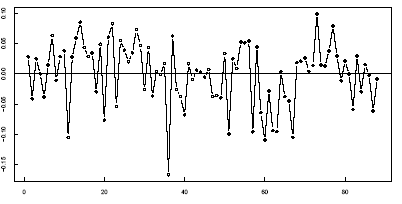
\epsfig{file= ../FIGURES/Group1_U.ps, width=12cm, height=6cm,
    bbllx=38, bblly=49, bburx=562, bbury=293, clip=}
  \end{tabular} \\
  \begin{tabular}{p{10cm}}
    Comparison \textred{individual} / multiple segmentation. \\
    \\
    The breakpoints detected around position 37 vanish.
  \end{tabular}
  &
  \begin{tabular}{l}
    \epsfig{file= ../FIGURES/Exemple_profile6_group1.ps, width=12cm,
    height=6cm, bbllx=65, bblly=65, bburx=560, bbury=182, clip=} 
  \end{tabular}
\end{tabular}

%%%%%%%%%%%%%%%%%%%%%%%%%%%%%%%%%%%%%%%%%%%%%%%%%%%%%%%%%%%%%
%%%%%%%%%%%%%%%%%%%%%%%%%%%%%%%%%%%%%%%%%%%%%%%%%%%%%%%%%%%%%
\newpage
\chapter{Looking for common aberrations}
%%%%%%%%%%%%%%%%%%%%%%%%%%%%%%%%%%%%%%%%%%%%%%%%%%%%%%%%%%%%%
%%%%%%%%%%%%%%%%%%%%%%%%%%%%%%%%%%%%%%%%%%%%%%%%%%%%%%%%%%%%%

\noindent
\begin{tabular}{cc}
  \begin{tabular}{p{7.5cm}}
    To detect \emphase{aberrations associated to a disease}
    (e.g. bladder cancer), we look for aberrations that appear
    \emphase{'significantly'  often} among a set of patients.  \\ \\
  $X_{it}$ denotes the status of position $t$ for patient $i$:
  $$
  \begin{tabular}{rcrl}
    $X_{it}$ & = & \textblue{--1} & \textblue{(loss)} \\
    & = & 0 & (normal) \\
    & = & \textred{+1} & \textred{(gain)}
  \end{tabular}
  $$
  \refer{Hupp� et al.}{2004}
  \end{tabular}
  &
  \begin{tabular}{c}
    \epsfig{file=/RECHERCHE/RUPTURES/Etudes/Curie/MinRegion/Data1/Profiles.eps,
    }
  \end{tabular}
\end{tabular}

% %%%%%%%%%%%%%%%%%%%%%%%%%%%%%%%%%%%%%%%%%%%%%%%%%%%%%%%%%%%%%%%%%%%%%%
% \newpage
% \section{Discretized CGH profiles}
% %%%%%%%%%%%%%%%%%%%%%%%%%%%%%%%%%%%%%%%%%%%%%%%%%%%%%%%%%%%%%%%%%%%%%%

% \hspace{-2cm}
% \begin{tabular}{cc}
%   \begin{tabular}{p{7cm}}
%     $i = 1..m$ patients \\
%     ($m = 84$), \\
%     \\
%     $t = 1..n$ positions \\
%     ($n = 2360$) \\
%     \\
%     $X_{it}$ = status of\\
%     patient $i$ %\\
%     at position $t$. \\
%     \\
%     \begin{tabular}{rcrl}
%       $X_{it}$ & = & \textblue{--1} & \textblue{(loss)} \\
%        & = & 0 & (normal) \\
%        & = & \textred{+1} & \textred{(gain)}
%     \end{tabular}
%   \end{tabular}
%   &
%   \begin{tabular}{c}
%     \epsfig{file=/RECHERCHE/RUPTURES/Etudes/Curie/MinRegion/Data1/Profiles.eps}
%   \end{tabular}
% \end{tabular}

%%%%%%%%%%%%%%%%%%%%%%%%%%%%%%%%%%%%%%%%%%%%%%%%%%%%%%%%%%%%%%%%%%%%%%
\newpage
\section{Minimal region}
%%%%%%%%%%%%%%%%%%%%%%%%%%%%%%%%%%%%%%%%%%%%%%%%%%%%%%%%%%%%%%%%%%%%%%

\begin{tabular}{cc}
  \begin{tabular}{p{15cm}}
    A minimal region is a sequence of \emphase{successive positions}
    for which the \emphase{same status} is observed in \emphase{large
    number} of patients at the same time. \refer{Rouveirol}{2007}\\
    \\
    \paragraph{Data.} $M^* = 31$ patients present $\ell =
    5$ successive deletions between positions 1189 and 1193, in
    chromosome 9. \\
    \\
    \paragraph{Question.} Is this significant, given the number of
    patients ($m=84$) and the profiles length ($n=2340$)?
%     It is characterized by
%     \begin{itemize}
%     \item its position $t^* \in \{1..n\}$, 
%     \item its length $\ell$,
%     \item its status $s \in \{-1, 0, +1\}$, 
%     \item the number of patients $M^* \in \{1..m\}$.
%     \end{itemize} \\
  \end{tabular}
  &
  \begin{tabular}{c}
    \epsfig{file=/RECHERCHE/RUPTURES/Etudes/Curie/MinRegion/Data1/ExMinRegion.eps,
      clip=, bbllx=270, bblly=209, bburx=400, bbury=593}
  \end{tabular}
\end{tabular}


%%%%%%%%%%%%%%%%%%%%%%%%%%%%%%%%%%%%%%%%%%%%%%%%%%%%%%%%%%%%%%%%%%%%%%
\newpage
\section{Motifs are back}
%%%%%%%%%%%%%%%%%%%%%%%%%%%%%%%%%%%%%%%%%%%%%%%%%%%%%%%%%%%%%%%%%%%%%%

\paragraph{Binary case.} Assume that only 2 status exist: 
$$
X_{it} = \left\{ 
  \begin{array}{rl}
    1 & \mbox{for aberration,} \\
    0 & \mbox{for normal.}
  \end{array}
\right.
$$

\paragraph{Region.} A minimal region is then a $\ell$-run of
1s. Denote
$$
Y_{it} = \prod_{u=t-\ell+1}^t X_{it} = \left\{ 
  \begin{array}{rl}
    1 & \mbox{if a $\ell$-run occurs at position $t$ in profile $i$,} \\
    0 & \mbox{otherwise.}
  \end{array}
\right.
$$
% $Y_{it} = Y_{it}(\Rcal)$ indicates the
% occurrence of $\ell$ successive aberrations ending at position $t$ in
% patient $i$:
% $$
% Y_{it}= \prod_{u=1}^{\ell} X_{i, t-u+1}.
% $$
\paragraph{Simultaneous occurrences.} $Y_{+t} = \sum_i Y_{it}$ is
the number of patients for which a $\ell$ successive aberrations
(\emphase{$\ell$-run}) occurs at $t$.

\bigskip
\paragraph{Significance of an observed minimal region.} We have to calculate
$$
\Pr\left\{\max_{\ell \leq t \leq n}Y_{+t} \geq M^*\right\}.
$$

%%%%%%%%%%%%%%%%%%%%%%%%%%%%%%%%%%%%%%%%%%%%%%%%%%%%%%%%%%%%%%%%%%%%%%
\newpage
\section{Markov Model}
%%%%%%%%%%%%%%%%%%%%%%%%%%%%%%%%%%%%%%%%%%%%%%%%%%%%%%%%%%%%%%%%%%%%%%

\paragraph{Model.} 
Each profile $\{X_{it}\}_t$ is a 2-state stationary Markov chain (MC):
$$
\{X_{it}\}_t \sim \text{MC}(\Pibf, \mubf)
$$
where $\Pibf$ is the transition matrix and $\mubf$ the stationary
distribution ($\forall i: X_{i1} \sim \mubf$).

The patients (profiles) are supposed to be independent.

\bigskip
\paragraph{Estimated transition probabilities and stationary
  distributions.} States $= \{0, 1\}$:
$$
\text{Gain:} \qquad\qquad
\widehat{\Pibf}^+ = \left(\begin{array}{rr}
       99.74 &      0.26 \\
        1.98 &      98.02 \\
  \end{array}\right), 
\qquad \widehat{\mubf}^+ = (88.36 \quad      11.64), 
$$
$$
\text{Loss:} \qquad\qquad
\widehat{\Pibf}^- = \left(\begin{array}{rr}
        99.72 &      0.28 \\
       2.26 &       97.74 \\
  \end{array}\right), 
\qquad \widehat{\mubf}^- = (88.98 \quad      11.02).
$$
% $$
% \widehat{\Pibf} = \left(\begin{array}{rr}
%        99.7 & 0.3 \\
%        2.0 &  98.0 \\
%   \end{array}\right), 
% \qquad \widehat{\mubf} = (88.4 \quad  11.6).
% $$

%%%%%%%%%%%%%%%%%%%%%%%%%%%%%%%%%%%%%%%%%%%%%%%%%%%%%%%%%%%%%%%%%%%%%%
\newpage
\section{Significance}
%%%%%%%%%%%%%%%%%%%%%%%%%%%%%%%%%%%%%%%%%%%%%%%%%%%%%%%%%%%%%%%%%%%%%%

We want to evaluate 
\vspace{-0.55cm}
$$
\Pr\left\{\max_{\ell \leq t \leq n}Y_{+t} \geq M^*\right\}.
$$

\paragraph{Exact calculation.} 
We need to consider $m$ independent Markov chains of order $\ell-1$:
\\
\centerline{$m = 84, \quad \ell = 15 \quad \rightarrow \quad 8.3\;
  10^{86}$ states...}

\bigskip
\paragraph{Upper bound.} 
Denoting $X_{+t} = \sum_i X_{it}$, we have
$$
\Pr\left\{\max_{\ell \leq t \leq n}Y_{+t} \geq M^*\right\} \leq
\Pr\{X_{+t}, X_{+, t+1}, \dots X_{+, t+\ell-1} \geq M^*\}.
$$
The latter probability can be calculated via an \emphase{embedded
  Markov Chain}.

\bigskip
\paragraph{Lower bound.} A lower can also be derived, using another
technique. \refer{R. et al.}{?}

%%%%%%%%%%%%%%%%%%%%%%%%%%%%%%%%%%%%%%%%%%%%%%%%%%%%%%%%%%
\newpage
\subsection{Bladder cancer}

Deleted regions in $m = 84$ patients, $n = 2340$ positions along 24
chromosomes.
$$
\begin{tabular}{cccccc}
  position &  & length & \# patients &
  \multicolumn{2}{c}{Significance} \\
  $t^*$  &  chrom.  &  $\ell$  &  $M^*$  &  $p$(upper)  &  $p$(lower) \\ 
\hline 
1189 & 9 & 5 & 31 & 6.04\;e--8 & 4.05\;e--8 \\ 
1387 & 11 & 3 & 30 & 6.82\;e--7 & 6.08\;e--7 \\ 
1430 & 11 & 3 & 27 & 5.08\;e--5 & 4.60\;e--5 \\ 
1340 & 10 & 22 & 23 & 1.18\;e--4 & 3.02\;e--6 \\ 
1457 & 11 & 3 & 26 & 1.91\;e--4 & 1.74\;e--4 \\ 
1006 & 8 & 42 & 21 & 4.95\;e--4 & 1.86\;e--8 \\ 
996 & 8 & 7 & 22 & 7.85\;e--3 & 4.78\;e--3 \\ 
584 & 4 & 6 & 19 & 1.82\;e--1 & 1.39\;e--1 \\ 
1947 & 17 & 26 & 16 & 2.33\;e--1 & 1.42\;e--2 \\ 
594 & 4 & 17 & 17 & 2.34\;e--1 & 5.16\;e--2 \\ 
643 & 5 & 11 & 17 & 4.18\;e--1 & 2.21\;e--1 \\ 

%   $t^*$  &  chrom.  &  $\ell$  &  $M^*$  &  $p$(upper)  &  $p$(lower) \\ 
\hline 
1340 & 10 & 22 & 18 & 5.75\;e--9 & 1.24\;e--11 \\ 
2347 & 24 & 13 & 17 & 1.80\;e--6 & 1.21\;e--7 \\ 
320 & 2 & 3 & 16 & 6.85\;e--4 & 5.93\;e--4 \\ 
1161 & 9 & 2 & 16 & 1.13\;e--3 & 1.09\;e--3 \\ 
1387 & 11 & 3 & 15 & 3.20\;e--3 & 2.80\;e--3 \\ 
1152 & 9 & 2 & 15 & 5.07\;e--3 & 4.87\;e--3 \\ 
996 & 8 & 7 & 13 & 1.42\;e--2 & 7.15\;e--3 \\ 
1413 & 11 & 2 & 13 & 7.52\;e--2 & 7.28\;e--2 \\ 
1690 & 13 & 2 & 13 & 7.52\;e--2 & 7.28\;e--2 \\ 
1430 & 11 & 3 & 12 & 1.72\;e--1 & 1.57\;e--1 \\ 
1688 & 13 & 2 & 12 & 2.32\;e--1 & 2.26\;e--1 \\ 
1455 & 11 & 5 & 11 & 2.94\;e--1 & 2.28\;e--1 \\ 

\end{tabular}
$$
\begin{itemize}
\item \vspace{-0.5cm} The \emphase{upper and lower bounds are close},
  except for long regions.
\item \vspace{-0.5cm} Deletions in chromosome 9 are \emphase{known to
    be associated to bladder cancer}.
\end{itemize}

%%%%%%%%%%%%%%%%%%%%%%%%%%%%%%%%%%%%%%%%%%%%%%%%%%%%%%%%%%
%%%%%%%%%%%%%%%%%%%%%%%%%%%%%%%%%%%%%%%%%%%%%%%%%%%%%%%%%%
\newpage
\chapter{What's next?}
%%%%%%%%%%%%%%%%%%%%%%%%%%%%%%%%%%%%%%%%%%%%%%%%%%%%%%%%%%
%%%%%%%%%%%%%%%%%%%%%%%%%%%%%%%%%%%%%%%%%%%%%%%%%%%%%%%%%%

\paragraph{Enriching the the multiple array model:}
\begin{itemize}
\item \vspace{-0.5cm} Classify the segments into status
\item \vspace{-0.5cm} Account for possible covariates (regarding the
  probes or the patients)
\item \vspace{-0.5cm} Maximum likelihood for the \emphase{complete
    model} including segmentation, classification, random effects and
  covariates seems \emphase{intractable}. \\
  $\rightarrow$ Approximations (\emphase{variationnal approaches}) are
  promising.
\end{itemize}
A \emphase{R package} should be available soon.

\bigskip\bigskip
\paragraph{Recent or new technologies:}
\begin{itemize}
\item \vspace{-0.5cm} High density: tiling arrays ($\simeq 10^5$
  probes per chromosomes)
\item \vspace{-0.5cm} High throughput sequencing (discrete signal).
\end{itemize}

% \begin{itemize}
% \item At this time, we do not perform classification in multiple array
%   analysis. We would have to deal with \emphase{two unobserved
%     structure}:
%   $$
%   \Ybf = \Tbf \textred{\Cbf} \mbf + \Zbf \textred{\Ubf} + \Ebf
%   $$
%   The EM algorithm involves to complicated calculations 
%   $\rightarrow$ \emphase{Variationnal approach?}
% \item \emphase{Covariates} can be added for free in the multiple
%   segmentation, via a regression term
%   $$
%   \Ybf = \textred{\Xbf} \Thetabf + \Tbf \mubf + \Zbf \Ubf + \Ebf
%   $$
% \item Assuming that the probe effects are fixed, would allow to
%   perform classification:
%   $$
%   \Ybf = \Tbf \textred{\Cbf} \mbf + \Zbf \textred{\Thetabf} + \Ebf
%   $$
% \end{itemize}

%%%%%%%%%%%%%%%%%%%%%%%%%%%%%%%%%%%%%%%%%%%%%%%%%%%%%%%%%%
\newpage
%%%%%%%%%%%%%%%%%%%%%%%%%%%%%%%%%%%%%%%%%%%%%%%%%%%%%%%%%%

\noindent
\begin{tabular}{ccc}
  \begin{tabular}{p{10cm}}
    \subsection{Collaborations}
    \\ \\ \\ 
    Institut Curie: \\
    \paragraph{F. Radvanyi, O. Delattre} \\
    \\
    Cancer center, San Francisco: \\
    \paragraph{C. Vaisse} \\
    \\
    INRA - URGV, Evry: \\
    \paragraph{J.-P. Renou} \\
    \\ \\ \\ \\ \\ \\ \\ \\
  \end{tabular}
  & &
  \begin{tabular}{p{12cm}}
    UMR AgroParisTech / INRA 518: \\
    \paragraph{E. Lebarbier, J-J. Daudin, B. Thiam} \\
    \\
    UMR CNRS 5558, Lyon: \\
    \paragraph{F. Picard}\\
    \\
    Masaryk univ.,  R�p. Tch�que: \\
    \paragraph{E. Budinska}\\
    \\
    Univ. Paris X: \\
    \paragraph{L. Pierre} \\
    \\
    Univ. Paris XI: \\
    \paragraph{M. Lavielle} \\
    \\
    LIPN, UMR CNRS 7030: \\
    \paragraph{C. Rouveirol} \\
    \\
    Western Australia univ: \\
    \paragraph{V. Stefanov}
  \end{tabular}
\end{tabular}

%%%%%%%%%%%%%%%%%%%%%%%%%%%%%%%%%%%%%%%%%%%%%%%%%%%%%%%%%%%%%%%%%%%%%%
%%%%%%%%%%%%%%%%%%%%%%%%%%%%%%%%%%%%%%%%%%%%%%%%%%%%%%%%%%%%%%%%%%%%%%
%%%%%%%%%%%%%%%%%%%%%%%%%%%%%%%%%%%%%%%%%%%%%%%%%%%%%%%%%%%%%%%%%%%%%%
%%%%%%%%%%%%%%%%%%%%%%%%%%%%%%%%%%%%%%%%%%%%%%%%%%%%%%%%%%%%%%%%%%%%%%
\end{document}
%%%%%%%%%%%%%%%%%%%%%%%%%%%%%%%%%%%%%%%%%%%%%%%%%%%%%%%%%%%%%%%%%%%%%%
%%%%%%%%%%%%%%%%%%%%%%%%%%%%%%%%%%%%%%%%%%%%%%%%%%%%%%%%%%%%%%%%%%%%%%
%%%%%%%%%%%%%%%%%%%%%%%%%%%%%%%%%%%%%%%%%%%%%%%%%%%%%%%%%%%%%%%%%%%%%%
%%%%%%%%%%%%%%%%%%%%%%%%%%%%%%%%%%%%%%%%%%%%%%%%%%%%%%%%%%%%%%%%%%%%%%
